\documentclass[a4paper]{ltjsarticle}
\usepackage[no-math]{fontspec}
%% ブックマーク
\usepackage[unicode,hidelinks,pdfusetitle]{hyperref}
%% 和文フォント
%\usepackage[deluxe,yu-win10]{luatexja-preset}
\usepackage[deluxe,haranoaji]{luatexja-preset}
%% 画像
\usepackage{graphicx}
\usepackage{tikz,scsnowman}

\usepackage{listings}
\lstset{
        %プログラム言語(複数の言語に対応,C,C++も可)
        language = Python,
        %背景色と透過度
        backgroundcolor={\color[gray]{.90}},
        %枠外に行った時の自動改行
        breaklines = true,
        %自動改行後のインデント量(デフォルトでは20[pt]) 
        breakindent = 10pt,
        %標準の書体
        basicstyle = \ttfamily\scriptsize,
        %コメントの書体
        commentstyle = {\itshape \color[cmyk]{1,0.4,1,0}},
        %関数名等の色の設定
        classoffset = 0,
        %キーワード(int, ifなど)の書体
        keywordstyle = {\bfseries \color[cmyk]{0,1,0,0}},
        %表示する文字の書体
        stringstyle = {\ttfamily \color[rgb]{0,0,1}},
        %枠 "t"は上に線を記載, "T"は上に二重線を記載
        %他オプション:leftline,topline,bottomline,lines,single,shadowbox
        frame = TBrl,
        %frameまでの間隔(行番号とプログラムの間)
        framesep = 5pt,
        %行番号の位置
        numbers = left,
        %行番号の間隔
        stepnumber = 1,
        %行番号の書体
        numberstyle = \tiny,
        %タブの大きさ
        tabsize = 4,
        %キャプションの場所("tb"ならば上下両方に記載)
        captionpos = t
}

\usepackage{here}
\usepackage[hang,small,bf]{caption}
\usepackage[subrefformat=parens]{subcaption}
\captionsetup{compatibility=false}

%% タイトル
\title{My \TeX Template}
\author{@uwitty}

\begin{document}
% (以降文書本体)
\maketitle
\thispagestyle{empty}
\newpage

\pagenumbering{roman}

\begin{abstract}
近年文書作成の機会が多くなっており、
文書作成を効率的に行う必要性が増している。
\TeX は著名な組版ソフトウェアで、
簡易なテキスト(ソースコード)を入力するだけで、
綺麗に組版された文書が出力されることに定評がある \cite{bib:bibun9}。
しかし、組版のためのコマンドをテキストで入力する必要があり、
コマンド名やそれに与えるオプション設定等をいちいち覚えていられない等の課題がある。
コマンドや設定は毎回変える必要がないため、
何らかのテンプレートを予め用意しておき、
使い回せるようにしておくと大変便利である。
そこで、 
本レポートでは Lua\TeX \cite{bib:luatexjasite} を用いて文書作成するためのテンプレートをについて記述する。
\end{abstract}
\newpage

\tableofcontents

\newpage
\pagenumbering{arabic}

\section{導入}

\subsection{概要}

本レポートは、
Lua\TeX-ja \cite{bib:luatexjasite} を使用した文書作成用テンプレートである。
使用環境は Ubuntu 24.04 である。
preamble 冒頭は参考文献 \cite{bib:luatexpreamble} を、
listings パッケージの設定は参考文献 \cite{bib:lstsettings} を参考にした。

\subsection{環境構築}

Ubuntu 24.04 上で、関連パッケージをインストールするスクリプトを、
リスト \ref{lst:install} に示す。

\lstinputlisting[caption=インストールスクリプト (Ubuntu 24.04 用), label=lst:install, language=bash]{scripts/install.sh}

\subsection{用語}

本レポートで使用する用語 (を記述するためのテンプレート) を表 \ref{tbl:words} に示す。

\begin{table}[H]
\begin{center}
\caption{用語}
\begin{tabular}{llp{6cm}}
用語 & 説明 & 備考 \\
\hline
\TeX & 組版ソフト & - \\
\end{tabular}
\label{tbl:words}
\end{center}
\end{table}

\subsection{本文書の構成}

省略   

\newpage
\section{本文作成用テンプレート}

\subsection{画像}

画像を図 \ref{fig:bibun9paper} に示す。
Caption に footnote をつける例として、
取得元の URL を脚注に追加している。

\begin{figure}[H]
\begin{center}
%\hspace*{3cm}
        \includegraphics[height=8cm]{images/9784297138899.jpg}
        \caption{``LaTeX美文書作成入門" \cite{bib:bibun9} の書影 \footnotemark}
        \label{fig:bibun9paper}
\end{center}
\end{figure}
\footnotetext{\url{https://gihyo.jp/book/2023/978-4-297-13889-9}}

subfloat を使用して図を複数並べる例を図 \ref{fig:subfloats} に示す。
なお、図 \ref{fig:subfloats} \subref{subfig:tiger} の画像は、
参考文献 \cite{bib:tigereps} より取得したものを使用している。

\begin{figure}[H]
\centering
        \subfloat[][書影]{
                \includegraphics[height=4cm]{images/9784297138899.jpg}
                \label{subfig:bibun}
        } \quad
        \subfloat[][虎]{
                \includegraphics[height=4cm]{images/tiger.eps}
                \label{subfig:tiger}
        }
        \captionsetup{format=plain, font=large, margin=50pt}
        \caption{ロゴ: \subref{subfig:bibun} 書影 \subref{subfig:tiger} 虎}
        \label{fig:subfloats}
\end{figure}

同様の画像を用いて、
minipages を使用して図を複数並べる例を図 \ref{fig:minipages} に示す。

\begin{figure}[htbp]
  \begin{minipage}[b]{0.45\linewidth}
    \centering
    \includegraphics[keepaspectratio, height=4cm]{images/9784297138899.jpg}
    \subcaption{書影}
  \end{minipage}
  \begin{minipage}[b]{0.45\linewidth}
    \centering
    \includegraphics[keepaspectratio, height=4cm]{images/tiger.eps}
    \subcaption{虎}
  \end{minipage}
  \caption{minipage を使用して画像を並べて表示する例}
  \label{fig:minipages}
\end{figure}

\subsection{表}

表のサンプルを表 \ref{tbl:sample} に示す。

\begin{table}[H]
\centering
\caption{サンプル}
\begin{tabular}{crp{6cm}}
        項目 & 数値 & 備考 \\
        \hline
        a &    1 & 1つ目 \\
        b &   12 & - \\
        c &  123 & - \\
        d & 1,23 & - \\
\end{tabular}
\label{tbl:sample}
\end{table}

別パターンの表のサンプルを表 \ref{tbl:sample} に示す。

\begin{table}[H]
\centering
\caption{サンプル}
\begin{tabular}{crlp{6cm}}
        項目 & \multicolumn{2}{l}{数値} & 備考 \\
        \hline
        a &    1 & kg & 1つ目 \\
        b &   12 & mm & - \\
        c &  123 & 秒 & - \\
        d & 1,23 & & -  \\
\end{tabular}
\label{tbl:sample}
\end{table}

\subsection{リスト}

bash の例をリスト \ref{lst:bashsample} に示す。

\begin{lstlisting}[caption = Bash 例, label = lst:bashsample, language=bash]
#!/bin/bash
set -e -x

apt update
\end{lstlisting}

python の例をリスト \ref{lst:pythonsample} に示す。

\begin{lstlisting}[caption = Python ソースコード例, label = lst:pythonsample, language=python]
import sys

def main():
    print(*sys.argv, sep="\n")

if __name__ == '__main__':
    main()
\end{lstlisting}

c の例をリスト \ref{lst:csample} に示す。

\begin{lstlisting}[caption = C ソースコード例, label = lst:csample, language=c]
#include <stdio.h>

int main()
{
	printf("Hello, TeX. \n");
	return 0;
}
\end{lstlisting}


\subsection{作図}

参考文献 \cite{bib:tikzsample} より、
tikz による作図の例を図 \ref{fig:tikzsample} に示す。

\begin{figure}[htbp]
\centering
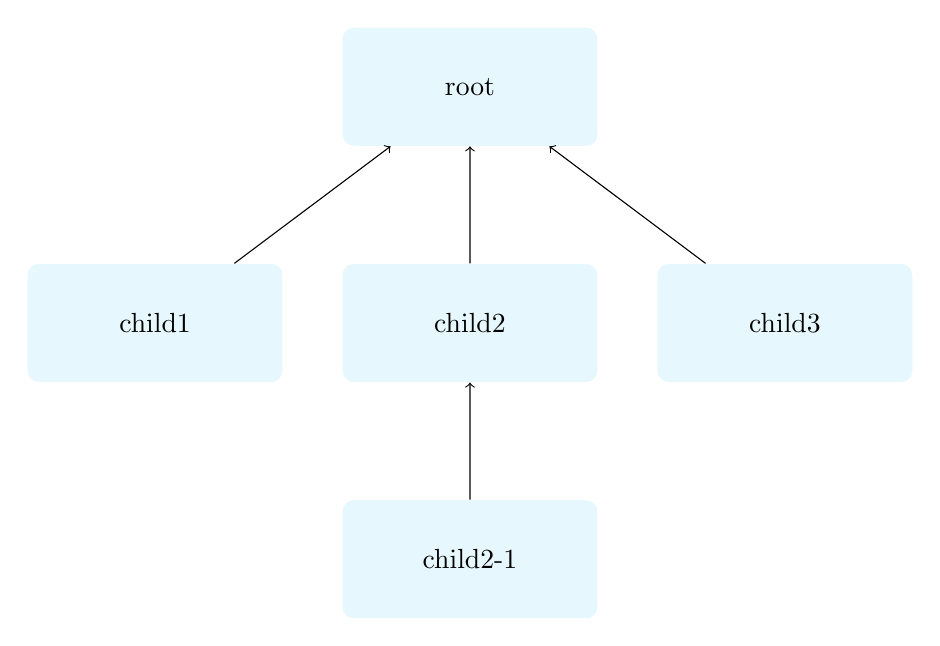
\begin{tikzpicture}
    \tikzset{block/.style={rectangle, fill=cyan!10, text width=3cm, text centered, rounded corners, minimum height=1.5cm}};
    \node[block] {root} [level distance=3cm, sibling distance=4cm, edge from parent/.style={<-,draw}]
        child{ node[block] {child1} }
        child{ node[block]{child2}
            child{ node[block]{child2-1} }
        }
        child{ node[block] {child3} };
\end{tikzpicture}
\caption{Tikz サンプル}
\label{fig:tikzsample}
\end{figure}


\newpage
\section{参考文献の記述}

\subsection{概要}

このテンプレートでは、
リスト \ref{lst:bibsettings} のように参考文献を挿入している。
参考文献に関する情報は bib ファイルに別途記述する。

\begin{lstlisting}[caption = 参考文献のスタイルと bib ファイル指定, label = lst:bibsettings]
%\bibliographystyle{jplain}
\bibliographystyle{junsrt}
\bibliography{ref}
\end{lstlisting}

参考文献はリスト \ref{lst:refbib} のように記述する。
ここでは、冒頭部分のみ示している。
Web サイトの引用は、
``SIST 科学技術情報流通技術基準" \cite{bib:sistref} を参考に、
@misc で記述している。
%https://warp.ndl.go.jp/info:ndljp/pid/12003258/jipsti.jst.go.jp/sist/index.html
bib エントリの詳細については\ref{sec:bibentry}を参照。

\lstinputlisting[caption=参考文献記述ファイル (ref.bib), label=lst:refbib, language=tex, lastline=14]{ref.bib}

\subsection{ビルド手順}

参考文献を追加してビルドする際の手順を、リスト \ref{lst:bibbuild} に示す。
Ubuntu 環境下では日本語用参考文献スタイルファイルのパスが参照されないため、
BSTINPUTS 環境変数に該当パスを追加して bibtexu コマンドを実行している。

\lstinputlisting[caption=参考文献を追加する際のビルド手順 (bibbuild.sh), label=lst:bibbuild, language=bash]{scripts/bibbuild.sh}

\newpage
\section{まとめ}

省略


\newpage
%\bibliographystyle{jplain}
\bibliographystyle{junsrt}
\bibliography{ref}

\appendix
\newpage
\section{bib ファイルの文献種類と設定項目}
\label{sec:bibentry}

bibtex 記述時の文献種類と設定項目について表 \ref{tbl:bibtexentry} に示す \cite{bib:bibtexentry}。

\begin{table}[H]
\begin{center}
\caption{参考文献の種類と設定項目}
\begin{tabular}{p{2cm}lp{4cm}p{5cm}}
文献種類                 & bibtex          & 必須項目 (エントリー)            & 任意項目 (エントリー) \\
\hline
学術論文                 & @article        & auther, title, journal year      & volume, number, pages, month, note \\
博士論文                 & @phdthesis      & author, title, school, year      & type, address, month, note \\
修士論文                 & @mastersthesis  & author, title, school, year      & type, address, month, note \\
プロシーディングス       & @proceedings    & title, year                      & editor, volume, number, series, address, month, organization, publisher, note \\
プロシーディングスの一部 & @inproceedings  & author, title, booktitle, year   & editor, volume, number, series, pages, address, month, organization, publisher, note \\
会議録                   & @conference     & author, title, booktitle, year   & editor, volume, number, series, pages, address, month, organization, publisher, note \\
書籍                     & @book           & author または editor, title, publisher, year & volume, number, series, address, edition, month, note \\
小冊子                   & @booklet        & title                            & author, howpublished, address, month, year, note \\
書籍の一部               & @inbook         & author または editor, title, chapter または pages, publisher, year & volume, number, series, type, address, edition, month, year \\
書籍の一部(表題あり)     & @incollection   & author, title, booktitle, publisher, year & editor, volume, number, series, type, chapter, pages, address, edition, month, note \\
マニュアル               & @manual         & title                            & author, organization, address, edition, month, year, note \\
技術報告書               & @techreport     & author, title, institution, year & type, number, address, month, note \\
未発表                   & @unpublished    & author, title, note              & month, year \\
その他                   & @misc           & なし                             & author, title, howpublished, month, year, note \\
\end{tabular}
\label{tbl:bibtexentry}
\end{center}
\end{table}

\end{document}
